\chapter{Funktionaaliset frontend-ohjelmistokehykset}
Tämän tutkielman tutkimuskohteiksi on valittu funktionaaliset reaktiiviset ohjelmistokehykset React-kirjasto ja
Elm-ohjelmointikieli. Tutkielma käsittelee React-kirjastoa ja Elm-kieltä yleisesti funtionaalisen ohjelmoinnin kannalta,
sekä tarkemmin sitä, miten teknologiat toteuttavat tilankäsittelyn ja mahdollistavatko ne sivuvaikutukset.

\section{Ohjelmistokehykset}
React on Facebookin ylläpitämä avoimen lähdekoodin käyttöliittymäkirjasto, jota käytetään tyypillisesti
JavaScript-kielen kanssa. React on alunperin julkaistu vuonna 2013, ja se on kirjoitushetkellä vuonna 2020 maailman
suosituin frontend-ohjelmistokehys. Sillä on kirjoitushetkellä noin yhdeksän miljoonaa viikoittaista latausta
NPM-palvelusta \cite{npmtrends}. React-kirjaston syntaksi on deklaratiivista, ja se mahdollistaa käyttöliittymän
pilkkomisen komponentteihin. React ei ota kantaa muihin tekniikkaratkaisuihin, vaan keskittyy pelkästään yksittäisen
DOM-puun hallitsemiseen. Ohjelmistokehittäjälle jää näin täysi valta valita muut teknologiat vapaasti. \cite{reactjs}

Elm on funktionaalinen ohjelmointikieli, joka käännetään JavaScript-kieleksi. Elmin on alunperin kehittänyt Evan
Czaplicki osana maisterin tutkielmaansa vuonna 2012. Elm ei ole tutkielman kirjoitushetkellä saavuttanut suurta
suosiota, vaan sen NPM-paketinhallinnan latausmäärä on vain noin kolmekymmentä tuhatta latausta viikossa
\cite{npmtrends}. Elm keskittyy web-pohjaisten graafisten käyttöliittymien deklaratiiviseen toteuttamiseen. Elm
kytkeytyy tavallisen HTML DOM-puun solmuun. Elm ei myöskään rajoita muita tekniikkaratkaisuja, kuten tyylikielen
valintaa, mutta Elm-koodissa on haastavampaa käyttää muilla kuin Elm-kielellä kirjoitettuja komponentteja ja kirjastoja.
\cite{elmlang}

\section{Funktionaalinen ohjelmointi}
React korostaa funktionaalista ohjelmointityyliä imperatiivisen ohjelmoinnin sijaan, mutta sallii kuitenkin kaiken
tavallisen imperatiivisen JavaScript-syntaksin. React ei pystykään välttämään muuttuvia arvoja tai sivuvaikutuksia mutta
rohkaisee silti ohjelmoimaan funktionaalisesti muun muassa tarjoamalla tilanhallinan, joka soveltuu funktionaaliseen
ohjelmointiin. \cite{reactjs}

Elm taas pyrkii olemaan puhtaasti funktionaalinen ohjelmointikieli eikä salli lainkaan esimerkiksi muuttuvia arvoja tai
epäpuhtaita funktioita. Elm ei myöskään salli tilanteita, jotka voisivat aiheuttaa ajonaikaisia virheitä, vaan pakottaa
virheiden käsittelyn funktionaalisesti datana. Elm-kielen ajonaikanen ohjelmistokehys abstrahoi pintapuolisesti kaikki
epäpuhtaudet sisällensä, joten Elm-kielellä toteutettu ohjelma on näennäisesti puhtaan funktionaalinen. \cite{elmlang}

\section{Funktionaalinen tilankäsittely}
React tukee lokaalia tilaa missä tahansa komponentissa, joka on ristiriidassa funktionaalisen paradigman kanssa. Tila
React-kirjastossa on kuitenkin muuttumaton datarakenne, jonka muuttaminen vaatii sen korvaamisen uudella datalla. Tilan
muokkaamiseen on perinteisesti käytetty React-kirjaston Component-luokan setState-metodia, joka ylikirjoittaa tilan.
Seuraavassa on esimerkki React-kirjaston setState-funktion käytöstä:
\begin{minted}{js}
// väärin
this.state.greeting = 'Moikku';
// oikein
this.setState({ greeting: 'Moikku' });
\end{minted}
React-kirjasto tukee nykyään vakiona myös epäpuhtauksia funktioiksi abstraktoivia koukkuja (engl. hooks), suomenkielinen
termi ei ole vakiintunut, mutta mielestäni ymmärrettävä. Koukut mahdollistavat esimerkiksi tilankäsittelyn puhtaassa
funktionaalisessa komponentissa, ilman että tarvitaan luokkaa. Esimerkki React-kirjaston useState-koukun käytöstä:
\begin{minted}{jsx}
const Example = () => {
  // greeting on tila, joka muuttuu reaktiivisesti
  // setGreeting on funktio, jonka kutsuminen muuttaa tilan
  const [greeting, setGreeting] = useState('Moikku');
  return (
    <h1>{greeting}</h1>
  );
}
\end{minted}

Funktionaalisen React-sovelluksen toteutukseen on tyypillistä käyttää funktionaaliselle ohjelmalle tyypillistä
tilamallia, jossa koko sovelluksen tilaa kuvataan yhdessä paikassa. Tämänkaltainen tilanhallinta yksinkertaistaa
ymmärtämään tilan muutosten vaikutusta sovellukseen. Tyypillinen tapa toteuttaa keskitetty tilanhallinta
funktionaalisesti on käyttää reducer-funktiota, joka palauttaa uuden tilan aiemman tilan ja tapahtuman perusteella.
Modernissa React-kirjastossa tämänkaltaista tilanhallintaa voidaan käyttää useReducer-koukun avulla. Vastaavan
toteutuksen tarjoaa myös kolmannen osapuolien toteutuksista suosituimpiin kuuluva Redux-kirjasto
\cite{functionalwebdev}. Yksinkertaisiin sovelluksiin on silti riittävää käyttää lyhyemmän syntaksin natiiveja
vaihtoehtoja, kuten perinteinen setState-toteutus ja useState-koukku. \cite{reactjs}

Elm-kielen arkkitehtuurissa tila on Model-nimisessä abstraktoidussa datamallissa. Model-tilan kuvaaminen ja
päivittäminen on hyvin samankaltaista, kuin React-kirjaston Redux-tilanhallinta. Reduxin kehitys on saanutkin
inspiraation Elm-kielen Model-tilanhallinnasta. Model-tilan muokkaaminen tapahtuu kutsumalla update-funktiota
message-parametrilla samankaltaisesti kuin Redux-kirjaston reducer-funktiossa. \cite{elmlang} Esimerkki Elmin tilan
toteutuksesta:
\begin{minted}{elm}
-- MODEL
type alias Model = Int

init : Model
init =
  0

-- UPDATE
type MSG = Increment | Decrement

update : Msg -> Model -> Model
update msg model =
  case msg of
    Increment ->
      model + 1
    Decrement ->
      model - 1
\end{minted}

Sekä React-kirjaston että Elm-kielen tilanhallinta on hyvin tyypillistä funktionaalista ohjelmointia. Kumpikaan
ohjelmistokehys ei suosittele muuttuvaa tilaa, vaan tilaa säilötään muuttumattomassa tietorakenteessa. React-kirjastossa
yksittäisellä komponentilla voi olla lokaali tila. Elm-kielessä kaikki tila on oltava yhdessä Model-rakenteessa, kuten
Reactissa on myös usein tyypillistä toteuttaa reducer-funktion avulla.

\section{Sivuvaikutukset}
Sivuvaikutukset ovat käytännössä pakollisia tosimaailman frontend-sovellukselle. Tyypillisiä sivuvaikutuksia
frontend-ohjelmassa ovat muun muassa ulkoisen datan hakeminen, tapahtumankuuntelijan asettaminen ja manuaalinen DOM-puun
muokkaaminen.

React sallii kaiken perinteisen JavaScript-syntaksin, kuten muuttujat ja sivuvaikutukselliset funktiot. Funktionaalinen
ohjelmointimalli vaatiikin React-ohjelmoijalta omaa tahtoa kirjoittaa ohjelma funktionaalisesti. React kuitenkin suosii
monella tavalla funktionaalista ohjelmointimallia. Moderni React suosii komponenttien toteuttamista niin kutsuttuina
funktiokomponentteina, joiden oma tila ja sivuvaikutukset on toteutettava funktionaalisilla ohjelmointitavoilla.
Funktiokomponentissa sivuvaikutuksen toteuttaminen vaatii useEffect-koukun käyttämistä, joka tekee sivuvaikutuksen
käsittelemisestä näennäisesti funktionaalista. \cite{reactjs}
\begin{minted}{jsx}
const Example = ({ cardId }) => {
  const [card, setCard] = useState(null);
  // aiheuttaa sivuvaikutuksen, joka hakee uuden datan
  // rajapinnasta kun cardId-parametri muuttuu.
  useEffect(() => {
    const newCard = api.getCardById(cardId);
    setCard(newCard);
  }, [cardId]);
  return (
    <Card card={card} />
  );
}
\end{minted}

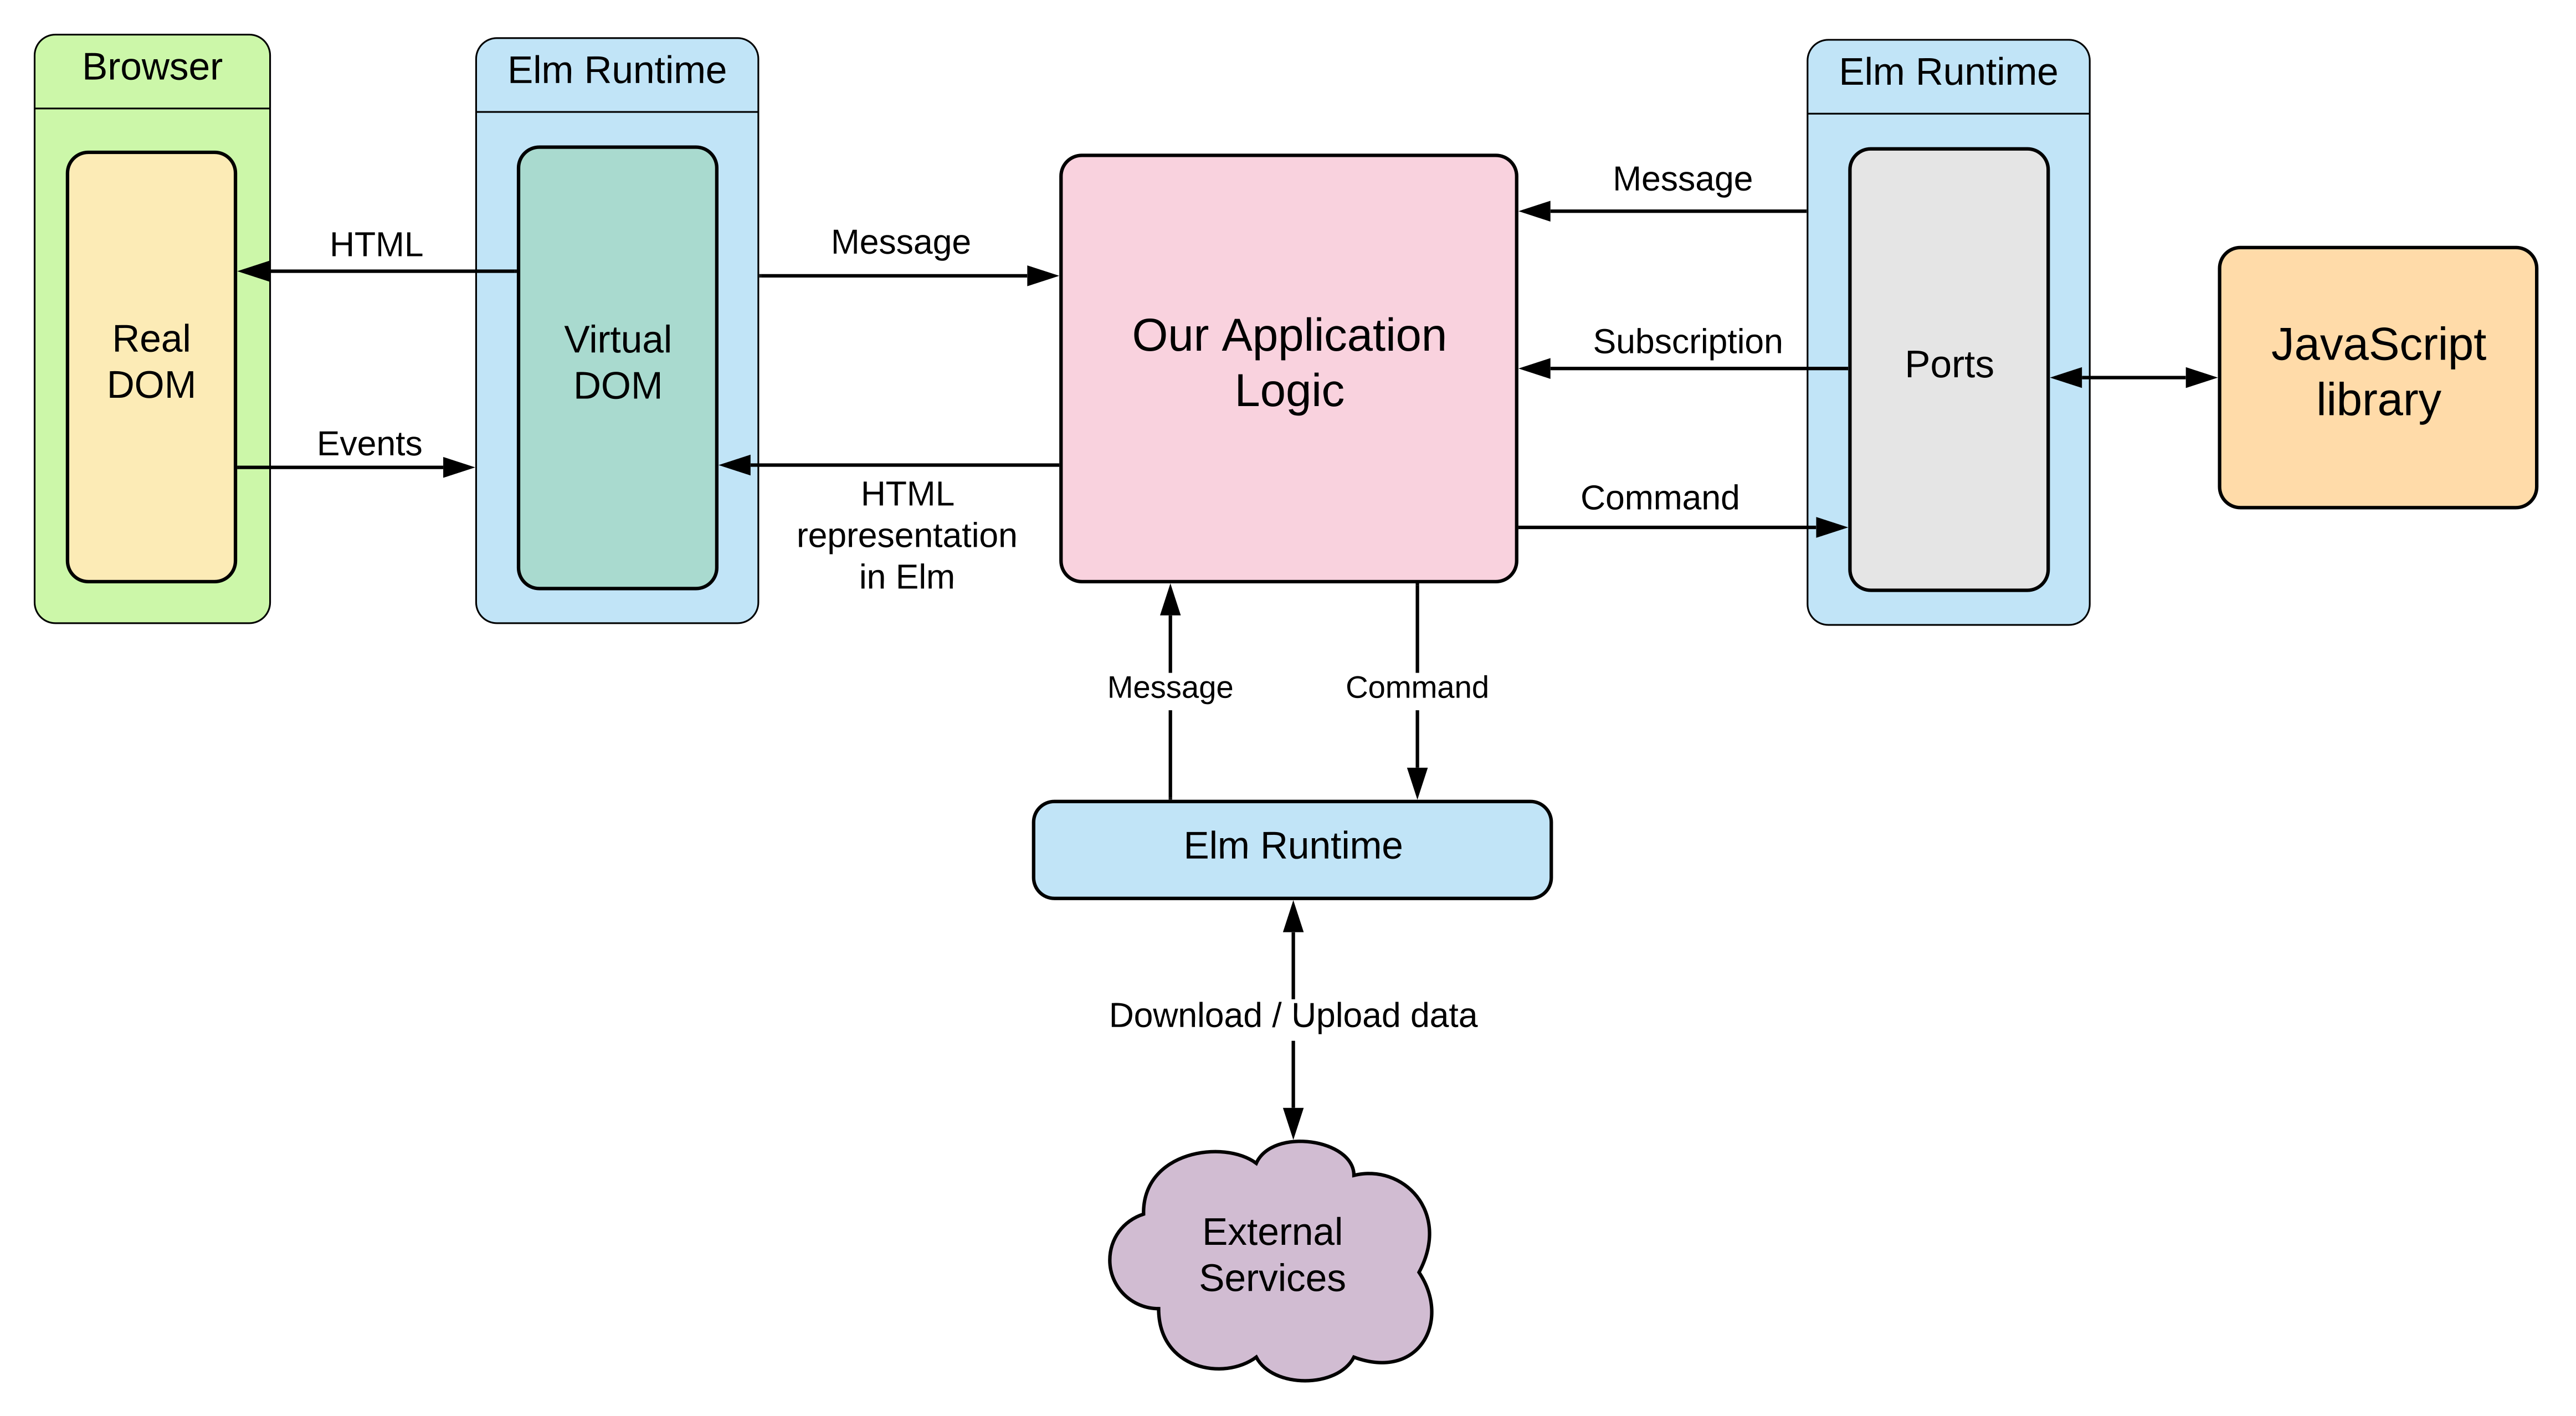
\includegraphics[width=\textwidth]{elm-runtime}
Elm-kieli ei salli epäpuhtauksia itse ohjelmakoodissa, vaan ne on kaikki toteutettava Elmin ajonaikaohjelmassa (engl.
Elm runtime). Näin itse ohjelma on puhtaasti funktionaalinen, mutta sivuvaikutuksellisia ohjelmia on silti mahdollista
kirjoittaa. Todellisuudessa Elm-kielen innokas laskentamalli aiheuttaa myös sivuvaikutuksia. \cite{elmlang}
